% \begin{abstract}
% Recent advances in large language models (LLMs) have sparked a new line of generative recommendation, where a model autogenerates a sequence of Semantic IDs (SIDs) instead of ranking a pre-selected candidate set.
% Although the current Supervised Fine-Tuning followed by Reinforcement Learning (SFT-then-RL) pipeline improves performance,
% it still suffers from (i) superficial SID understanding, because
% SFT merely forces the LLM to memorise a closed SID list,
% and (ii) coarse-grained rewards, as rule-based RL treats all incorrect SIDs
% equally.  
% We introduce \emph{SID-Navigated GEnerative Recommender} \textbf{(SINGER)}, a framework that injects fine-grained SID knowledge into every stage of the training process.  
% SINGER has two core components:  
% (1) Full-Process SID Alignment, which embeds alignment objectives
% throughout both SFT and RL to deepen the model’s grasp of the SID space; and  
% (2) SID-Guidance Reinforcement Learning, composed of
% SID-level rewards that grade a trajectory by the deepest correctly
% matched SID layer and SID-prefix curriculum sampling that supplies
% partial prefixes as intermediate hints for hard cases.  
% Experiments on public benchmarks demonstrate that SINGER
% consistently outperforms strong sequential, generative, and recent LLM-based baselines across standard metrics, validating the benefit of integrating hierarchical SID signals with the world knowledge of pretrained LLMs.
\begin{boxedabstract}

The recent success of large language models (LLMs) has sparked renewed interest in whether recommendation systems can enjoy similar scaling benefits.  
Conventional recommenders, dominated by massive embedding tables, often plateau as their dimensions grow, whereas the emerging generative recommendation paradigm replaces embeddings with compact \emph{Semantic ID} (SID) sequences produced by autoregressive Transformers.  
Yet, existing industrial deployments remain proprietary, leaving two fundamental questions unanswered: (\emph{i}) Do the anticipated scaling laws hold on public benchmarks? (\emph{ii}) What is the lightest post-training recipe that can unlock strong performance?

% This technical report introduces \textbf{MiniOneRec}, the first fully open-source framework for generative recommendation.  
\kxy{This technical report introduces \textbf{MiniOneRec}, the first fully open-source generative recommendation framework that provides an end-to-end workflow emcompassing SID generation, model SFT, and recommendation-driven RL.}
We construct SIDs via a Residual Quantized VAE and post-train Qwen backbones ranging from 0.5\,B to 7\,B parameters on the Amazon Review dataset.  
Our study reveals a clear downward trend in both training and evaluation negative as model size increases, confirming the parameter efficiency of the generative approach.  
To further boost performance, we propose a lightweight yet comprehensive post-training pipeline that (1) injects full-process SID alignment and (2) applies reinforcement learning with constrained decoding and hybrid rewards.  
Together, these techniques yield substantial gains in ranking quality and candidate diversity.  
Our codes are available at 
\url{https://github.com/AkaliKong/MiniOnRec}.

% 手动插入一张非浮动图
\end{boxedabstract}

%\begin{center}
%  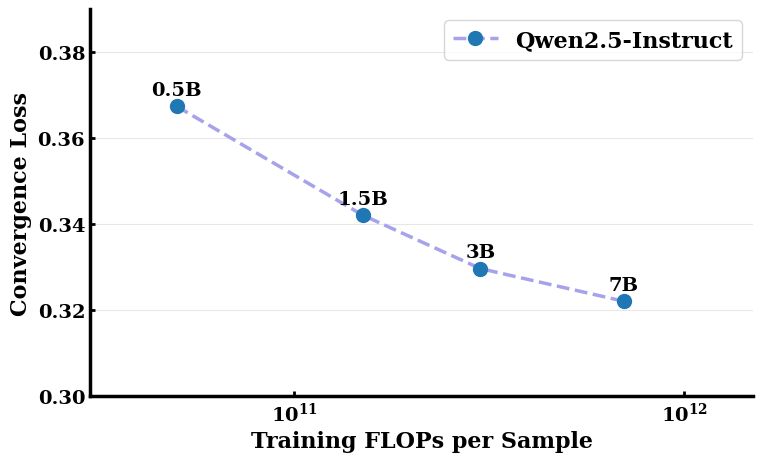
\includegraphics[width=0.7\textwidth]{figures/scaling.png}
%  \captionsetup{type=figure}       
%  \captionof{figure}{Scaling curves from 0.5B to 7B parameters.}
%  \label{fig:scaling}
%\end{center}

\begin{center}
\begin{minipage}[t]{0.40\textwidth}
\centering
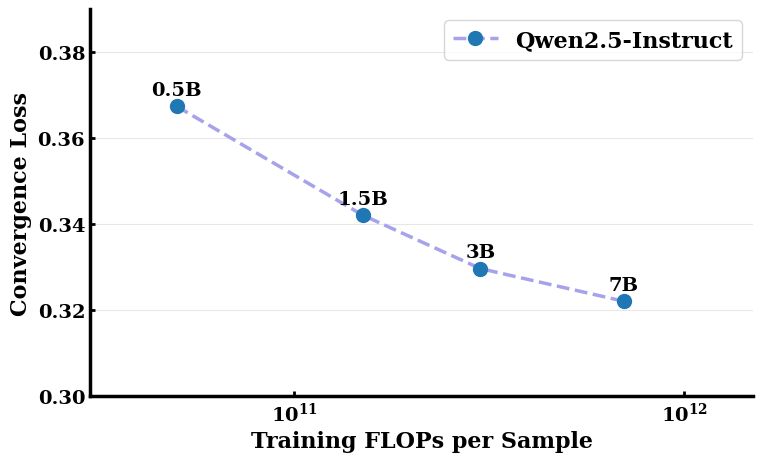
\includegraphics[width=\linewidth]{figures/scaling.png}
\end{minipage}\hfill
\begin{minipage}[t]{0.40\textwidth}
\centering
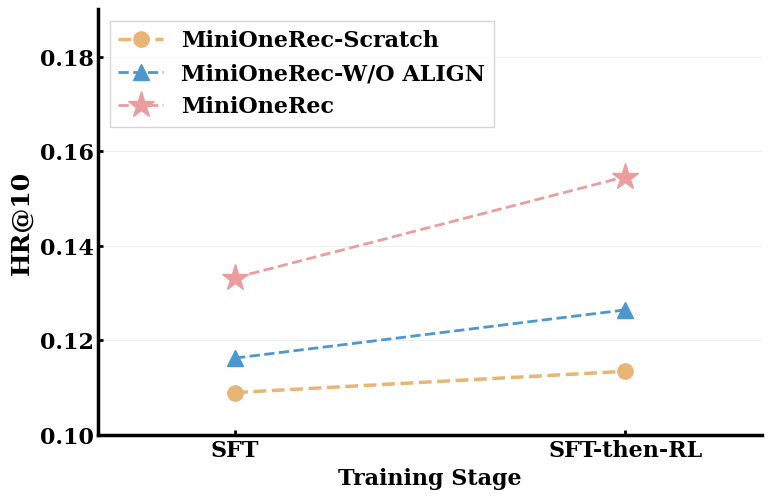
\includegraphics[width=\linewidth]{figures/llmmatter.png}
\end{minipage}
\captionsetup{type=figure}
\captionof{figure}{Scaling curves from 0.5B to 7B parameters.}
\label{fig:scaling}

\end{center}
% \end{abstract}

